\documentclass[11pt]{article}
\usepackage[margin=1in]{geometry}
\usepackage{amsmath,amssymb}
\usepackage{booktabs}
\usepackage{xcolor}
\usepackage{graphicx}
\usepackage{listings}
\usepackage[colorlinks=true,linkcolor=blue,urlcolor=blue,citecolor=blue]{hyperref}
\usepackage{parskip}

\definecolor{cset}{RGB}{31,119,180}
\definecolor{cfield}{RGB}{44,160,44}
\definecolor{cop}{RGB}{214,39,40}
\definecolor{cgray}{RGB}{120,120,120}

\newcommand{\code}[1]{\texttt{#1}}
\newcommand{\op}[1]{\textcolor{cop}{\texttt{#1}}}

\title{\textbf{The slime inverse problem in Plexus}\\[3pt]
\large Recovering the generating spec from a simulation}
\author{Janelia Research Campus}
\date{\today}

\begin{document}
\maketitle

\begin{abstract}
Plexus is a forward compiler: a small typed \emph{spec} (sets, fields, operators, a
schedule) is interpreted by a generic engine into a simulation, $\text{spec}\to
\text{engine}\to\text{trajectory}$. This note inverts that arrow. Given only a
simulation --- the cell positions and the chemical field over time --- we recover the
eight-number spec that generated it. We mirror each engine operator with a
\emph{differentiable} learnable operator validated exact against the engine, and fit
the parameters by gradient descent. One-step teacher forcing recovers the field and
motion parameters essentially exactly (about $224\times$ more accurate than a UCB
black-box search); a loss placed directly on \emph{particle positions} removes a
systematic bias in the sensing parameters; and moving from one cell type to two and
four makes the inter-type coupling \op{cross} --- unidentifiable for a single type ---
recoverable. The recovered specs do not reproduce a target pixel-for-pixel (the process
is stochastic) but reproduce it \emph{topologically}, which we argue is the correct
notion of success and which connects the rollout to generative diffusion models.
\end{abstract}

\section{From the forward model to its inverse}

The slime spec is eight continuous numbers: four on the field side
(\op{deposit}.amount, \op{diffuse}.rate, \op{decay}.rate, \op{sense}.cross) and four
per-cell motion parameters (move\_speed, turn\_speed, sensor\_angle, sensor\_dist).
The registered operators make every cell deposit into a chemical field, sense that
field at three forward sensors, turn toward the strongest reading, and advance; the
field meanwhile diffuses and decays. From a uniform-random start the population
condenses into the filament network of Fig.~\ref{fig:evo} (top). The \emph{inverse}
problem is $\text{trajectory}\to\text{spec}$: identify those eight constants from the
observed evolution alone.

\section{Method}

\textbf{Decomposed, engine-exact operators.} Each operator is mirrored by one
differentiable \code{nn.Module} whose parameters are tensors, and each carries a
self-test against the real engine: \op{deposit}, \op{diffuse}, \op{decay} and
\op{advance} match to $\le 10^{-7}$. \op{sense} is the one non-differentiable operator
(a hard three-way branch plus a random turn magnitude), so it is replaced by a smooth
mixture surrogate. A fit on these modules is therefore a fit on the real dynamics.

\textbf{One-step gradient descent.} The field is linear in its parameters, so a
single teacher-forced step $\text{field}_{t}\!\to\!\text{field}_{t+1}$ recovers
(amount, diffuse, decay) to $\sim\!10^{-3}$ and move\_speed from the displacement ---
where the black-box UCB baseline left \op{diffuse}.rate in the wrong half of its range.

\textbf{Loss on particles, not on reconstructed heading.} The sensing parameters were
at first recovered by matching a heading reconstructed as $\operatorname{atan2}$ of the
displacement, which biased \op{sense}'s sensor\_angle toward large values. Placing the
loss \emph{directly on the predicted particle positions} (free-run sense$\to$advance,
match where the cells are) removes the reconstruction and the bias; one-step beats a
recurrent rollout here, because the rollout accumulates chaos. Likelihood
\emph{profiles} --- scanning a parameter with the others fixed --- were the diagnostic
that distinguished ``biased objective'' from ``genuinely unidentifiable.''

\textbf{Multiple types.} With $C$ cell types the field carries $C$ channels and a cell
reads $(1-\text{cross})\,\cdot$ its own channel $+\,\text{cross}\cdot$ the total over
channels. The inter-type weight \op{cross} drives the multi-type dynamics and so
becomes identifiable, with accuracy improving as $C$ grows.

\section{Results: do we recover the parameters?}

Figure~\ref{fig:params} is the explicit answer, parameter by parameter (true in black,
recovered in green, values in the unit cube $u\in[0,1]$). For a single type the field
parameters and move\_speed are exact; turn\_speed, sensor\_angle and sensor\_dist
recover to a few percent; \op{cross} is \emph{held} because a single type cannot
constrain it. For four types every parameter including \op{cross} is recovered
(\op{cross} u-error $0.008$ at four types, $0.012$ at two). Across four random
single-type targets the sensor\_angle u-error is $0.015$/$0.158$/$0.092$/$0.051$ ---
the spread tracks how much lateral field structure each target presents to the sensors.

\begin{figure}[h]
\centering
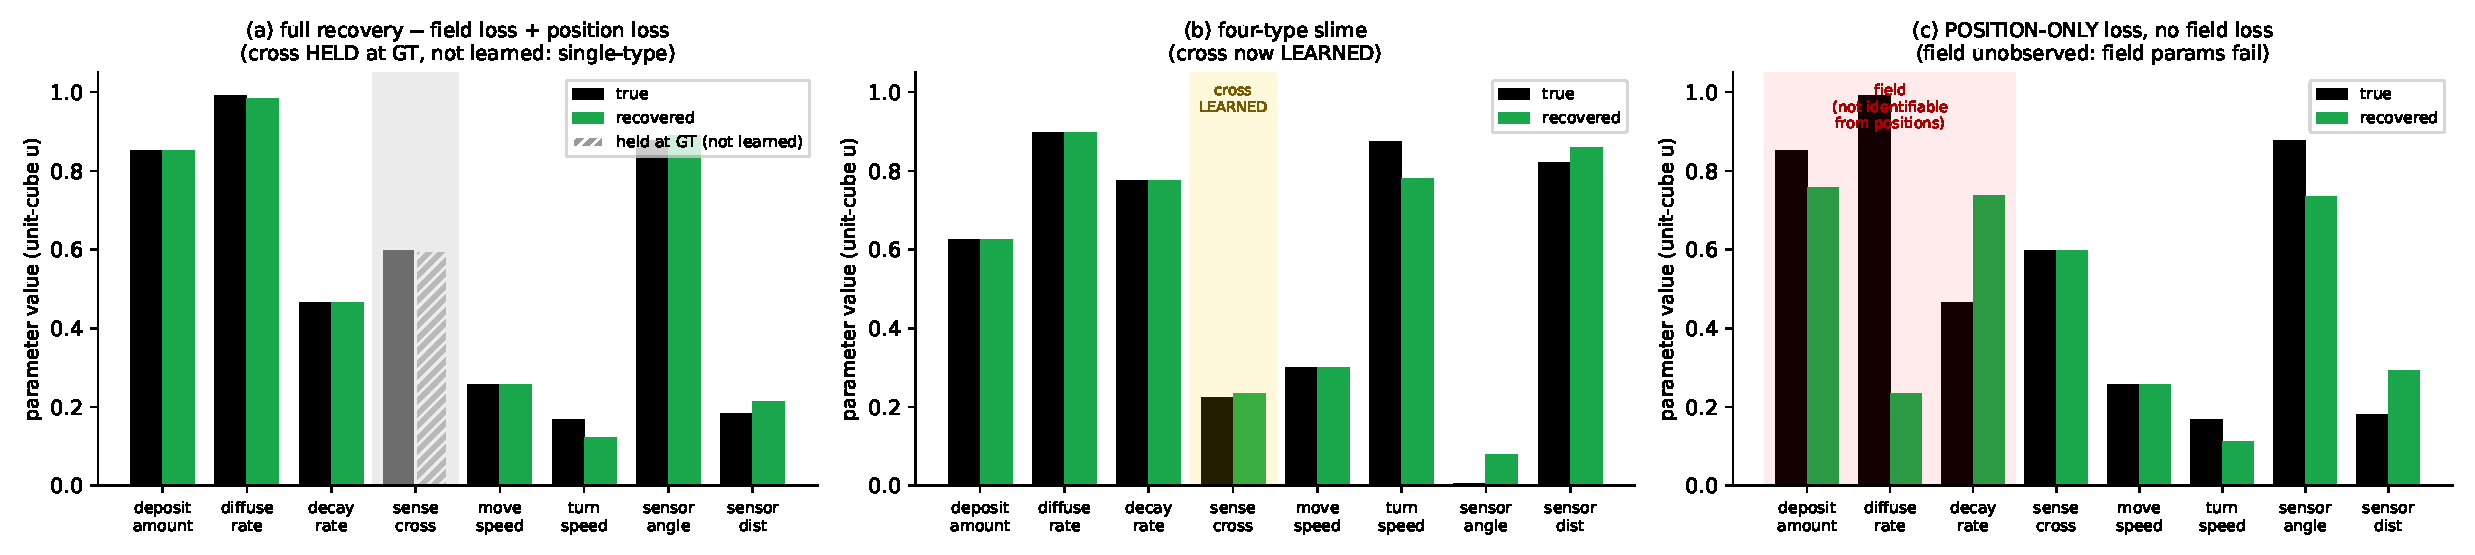
\includegraphics[width=\textwidth]{figures/fig_param_recovery.pdf}
\caption{\textbf{Parameter recovery, true vs.\ recovered} (unit-cube $u$; bars
\textbf{true} (black) vs \textbf{recovered} (green)). \textbf{(a)} single-type target,
field loss $+$ position loss: field and motion parameters recovered, but \op{cross} is
\emph{held} at its true value (grey hatched bar) --- a single type cannot constrain it,
so the matching bars are \emph{not} a recovery. \textbf{(b)} four-type slime: the same
scheme genuinely \emph{learns} \op{cross} (gold, green bar). \textbf{(c)} \emph{pure position-only loss with no field
loss} (the field is free-run and never observed): motion and sensing parameters still
recover, but the \emph{field} parameters (red) do \emph{not} --- they are unidentifiable
from particle motion alone over the usable horizon. This is the slime instance of the
cardio lesson: a latent field needs its own observation.}
\label{fig:params}
\end{figure}

\begin{figure}[h]
\centering
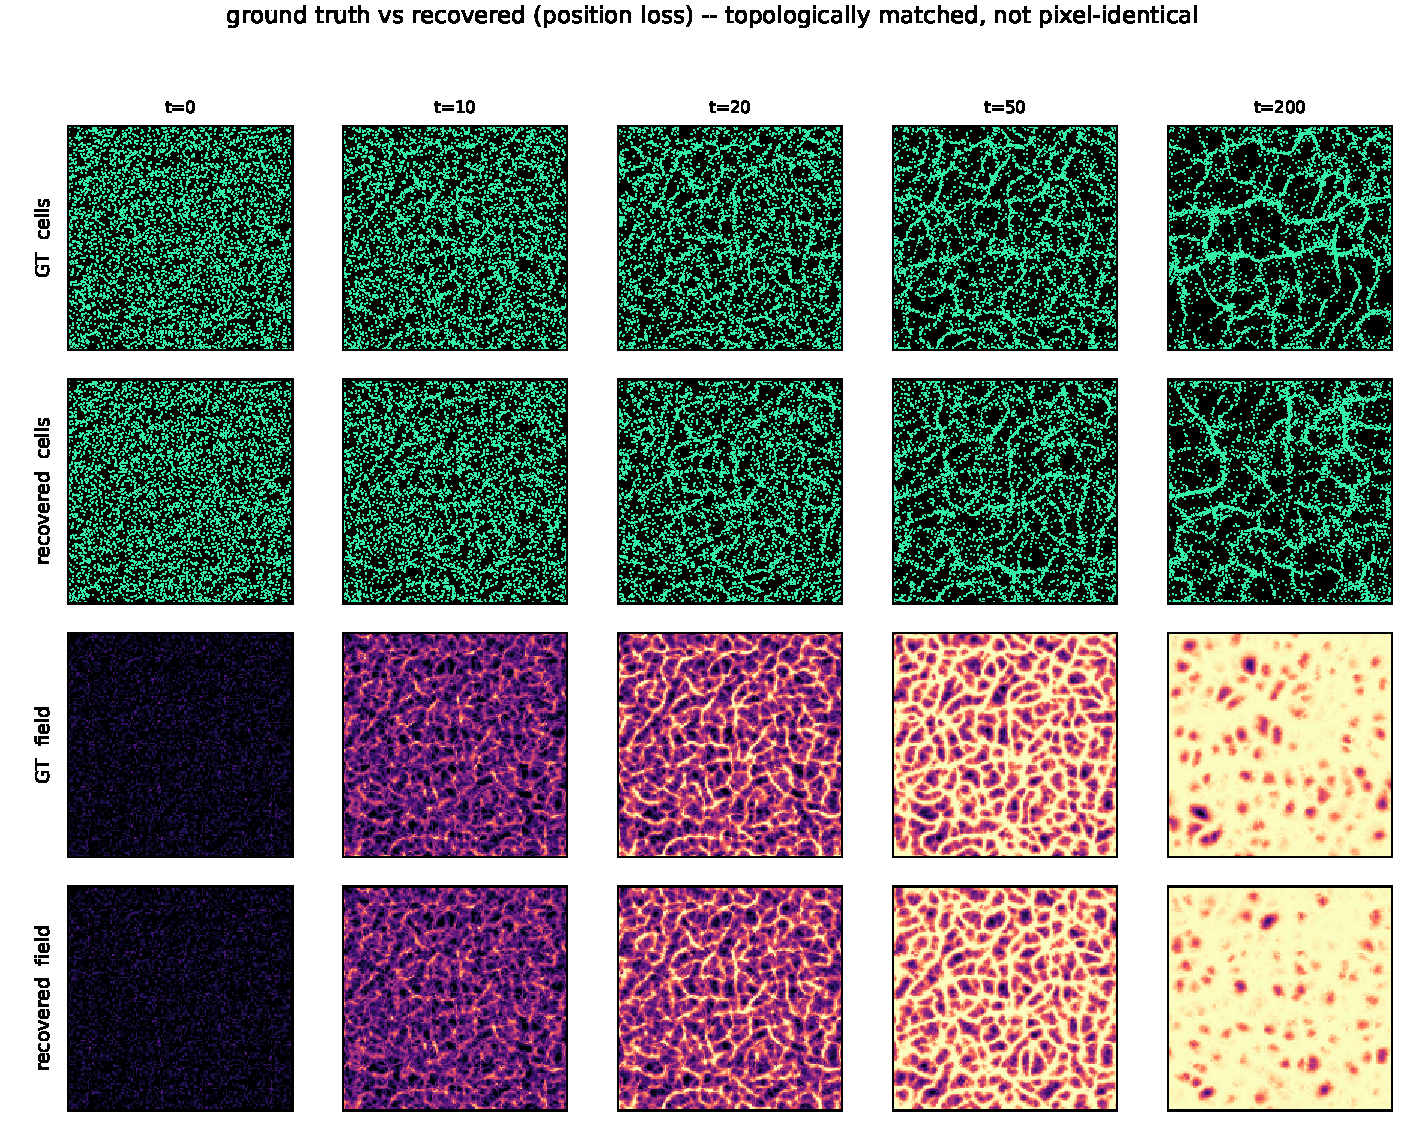
\includegraphics[width=\textwidth]{figures/fig_evolution.pdf}
\caption{\textbf{Ground truth vs.\ recovered} over time (cells, then the chemical
field). The recovered spec does not match the target frame-for-frame --- the process
is stochastic --- but produces the \emph{same topology}: the same filament network,
loop density and length scale.}
\label{fig:evo}
\end{figure}

\section{Three observations}

\paragraph{1. The rollout is a written generative process.} The time-lapse looks like a
generative diffusion model: each rollout starts from spatial \emph{noise} --- uniformly
random cell positions and an empty field --- and tick by tick condenses that noise into
a definite morphology, a path from noise to a sample on the data manifold. The decisive
difference is that the generative law is \emph{not} a learned black box: the transition
kernel $x_{t+1}=\Phi(x_t)$ is the explicitly written calculus of operators
(\op{deposit}, \op{diffuse}, \op{decay}, \op{sense}, \op{advance}), and the prior it
samples from is fixed by $\sim\!8$ interpretable constants. The inverse problem is
therefore not ``invert a neural sampler'' but ``identify the few physical constants of a
\emph{known} generative law,'' which is exactly why a handful of gradient steps suffice
where amortizing a diffusion prior would not. The stochasticity --- the random seed, the
random turn in \op{sense} --- plays the role of the diffusion noise schedule: any single
rollout is one sample, reproducible only in distribution, never pixel-for-pixel.

\paragraph{2. Parameters encode a topology, not a configuration.} This reframes what
``recovering the spec'' means. Two rollouts of the \emph{same} spec under different
seeds are never identical point-for-point, yet they are the same object topologically
--- the same kind of filament web, with the same branch density, loop statistics and
characteristic length. The parameters do not encode a particular configuration; they
encode a \emph{topology}, equivalently a \emph{dynamical regime} --- the attractor onto
which the operator flow condenses noise. Different parameter regions encode
qualitatively different topologies (a space-filling network vs.\ isolated clusters vs.\
a near-lattice), separated by bifurcations of the operator dynamics. So the inverse map
is really \emph{observed topology} $\to$ \emph{the dynamical law whose attractor has
that topology}, and our per-parameter identifiability findings are the precise statement
that some topological features pin some parameters (lateral field structure pins
sensor\_angle; multi-channel structure pins \op{cross}) while leaving others free.
Recovering the spec is recovering the \emph{generator} of a topology, not the topology
itself --- which is the version of the problem that is both well posed and useful.

\paragraph{3. Why the match is topological, not pointwise.} Because the success
criterion is distributional, the correct loss must be too. A pointwise position loss
works only on a short, pre-chaotic horizon; over long horizons the same spec decorrelates
from itself, and the only stable signal is the topology --- which is why behaviour-level,
permutation-invariant comparisons (and the per-frame, short-horizon position loss used
here) succeed where long pointwise rollouts fail. The encoded ``dynamics/topology'' is
thus the invariant the inverse problem is actually solving for.

\clearpage
\section*{Gallery: all ground-truth-vs-recovery panels}
\addcontentsline{toc}{section}{Gallery}
The panels below reproduce every visual page of \code{inverse\_gt\_vs\_stages.pdf}:
the showcase single-type target (method comparison), three further single-type
targets, and the two-type and four-type cases (cells coloured by type; the
multi-channel field shown as a per-species colour composite). In every panel the top
row is ground truth and the rows below are recoveries; columns are time.

\begin{figure}[p]\centering
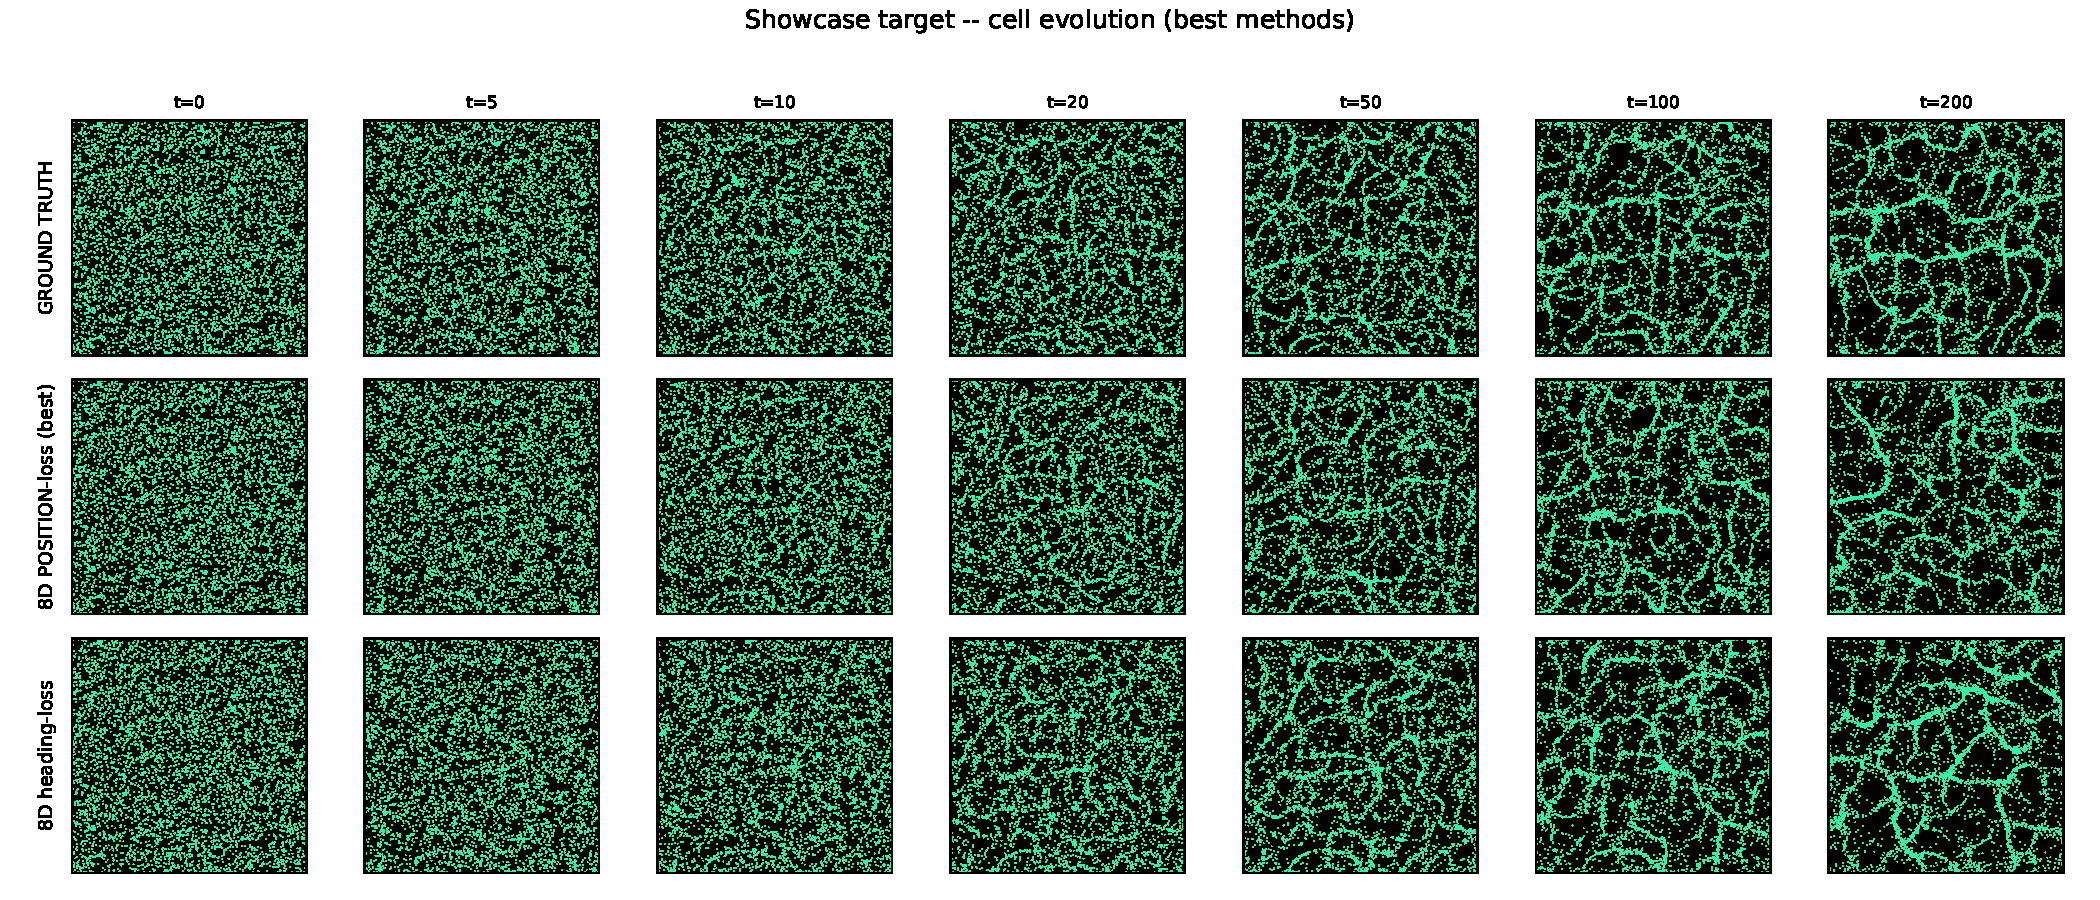
\includegraphics[width=\textwidth]{figures/gal_00.pdf}
\caption{Showcase single-type target, cell evolution: ground truth vs best methods.}
\end{figure}
\begin{figure}[p]\centering
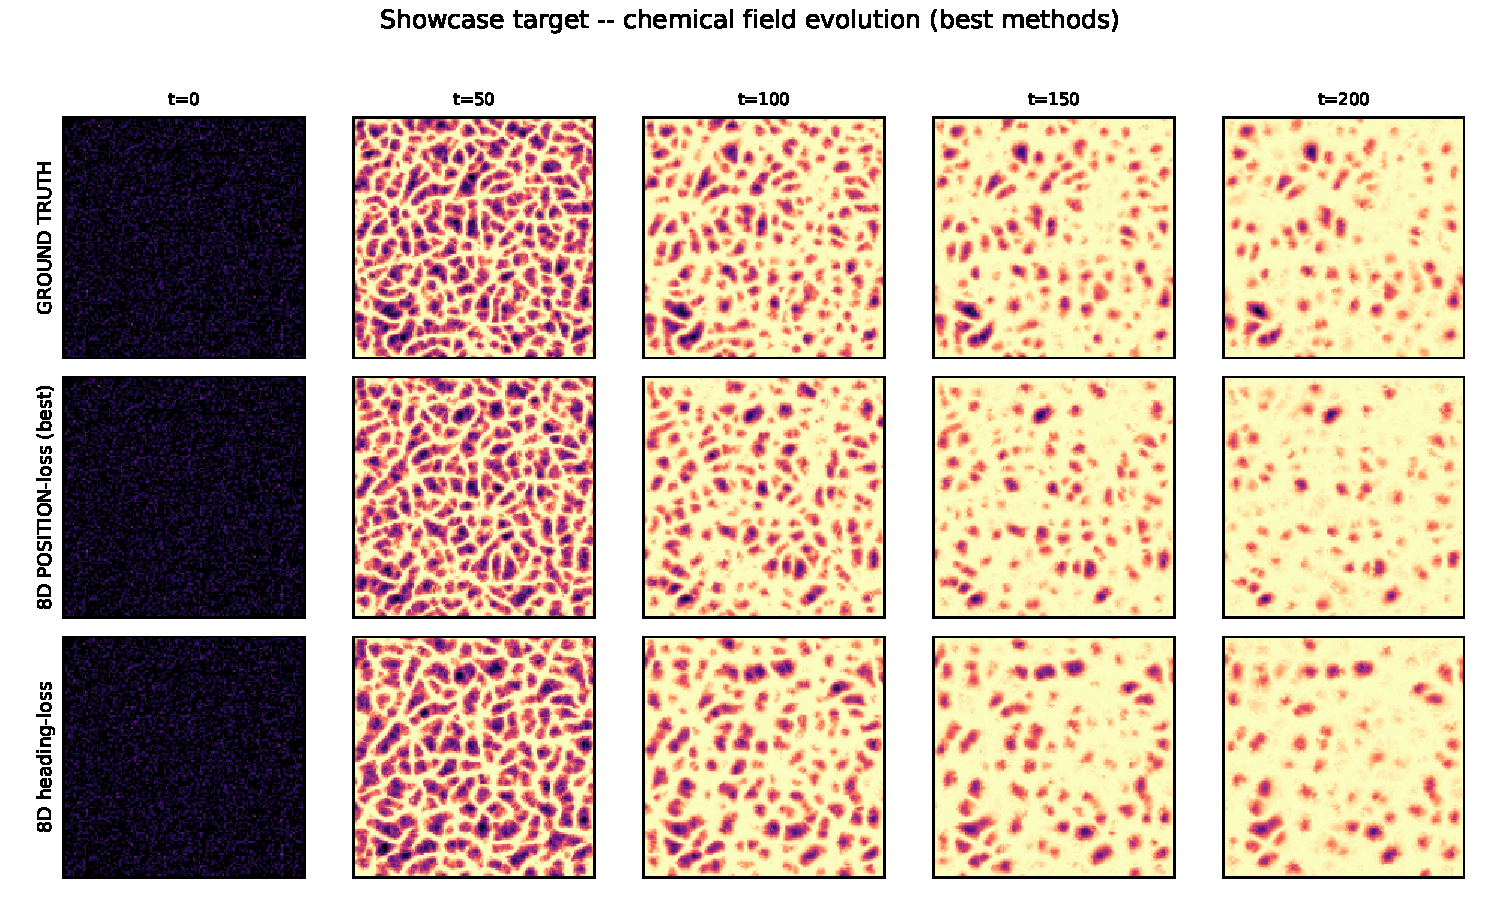
\includegraphics[width=\textwidth]{figures/gal_01.pdf}
\caption{Showcase single-type target, chemical field evolution: ground truth vs best methods.}
\end{figure}
\begin{figure}[p]\centering
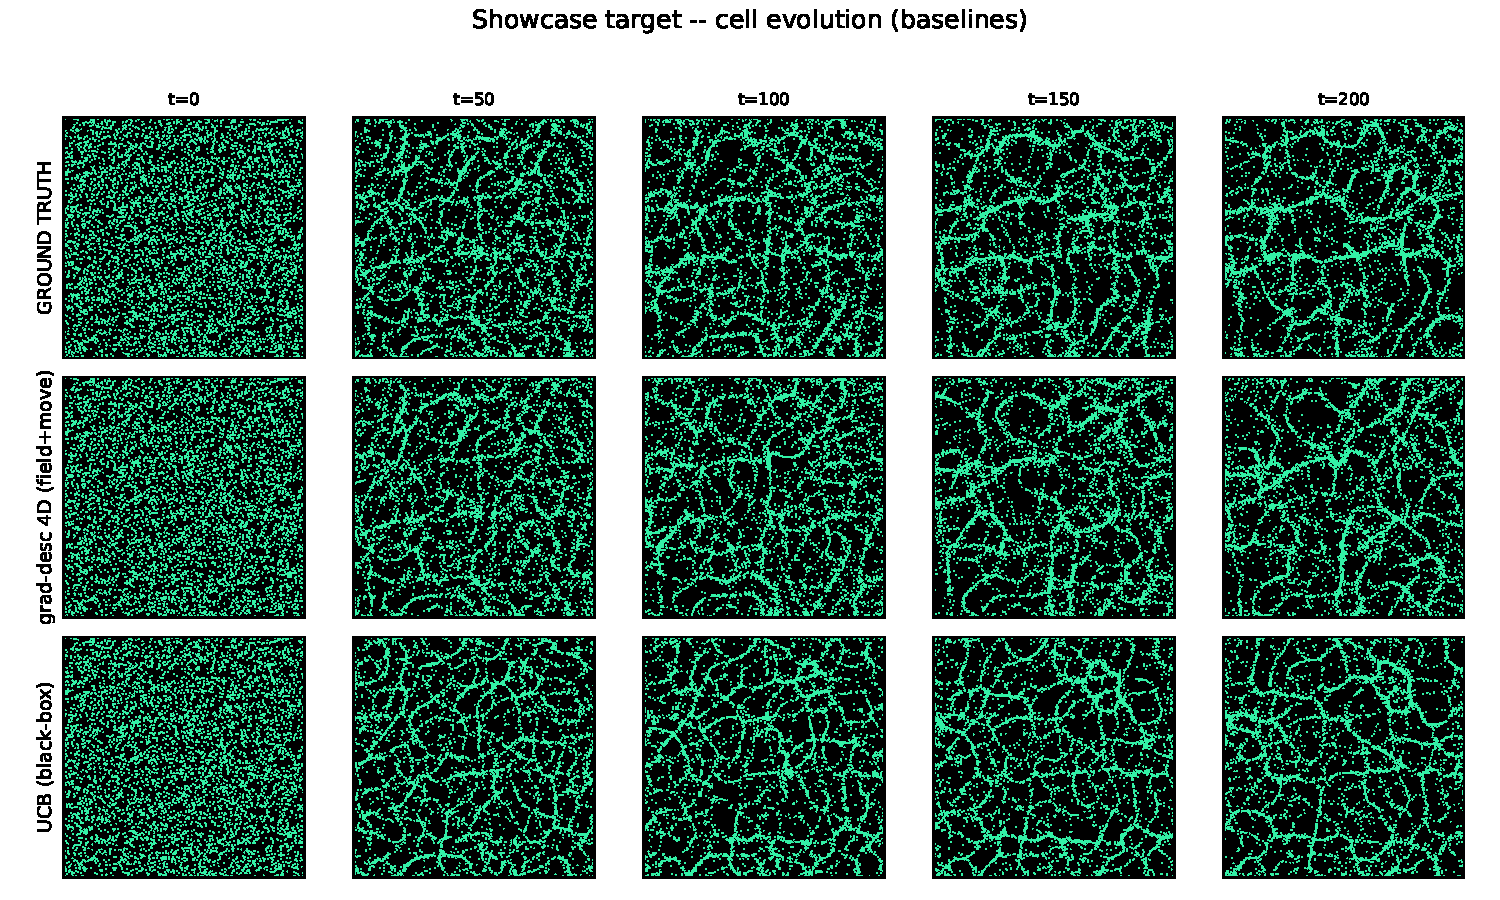
\includegraphics[width=\textwidth]{figures/gal_02.pdf}
\caption{Showcase single-type target, cell evolution: ground truth vs baselines.}
\end{figure}
\begin{figure}[p]\centering
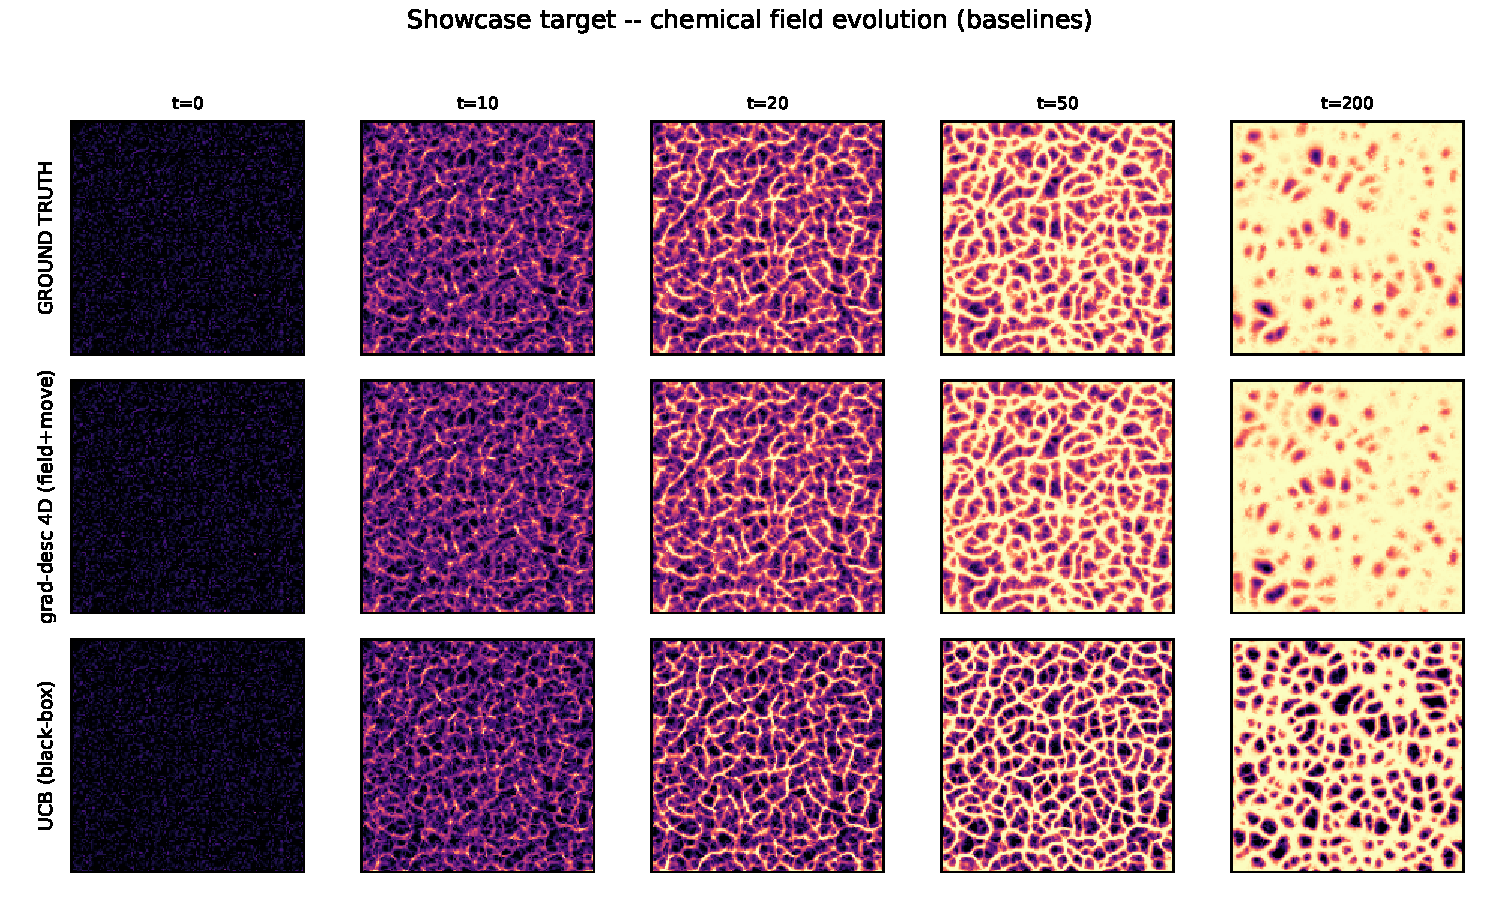
\includegraphics[width=\textwidth]{figures/gal_03.pdf}
\caption{Showcase single-type target, chemical field evolution: ground truth vs baselines.}
\end{figure}
\begin{figure}[p]\centering
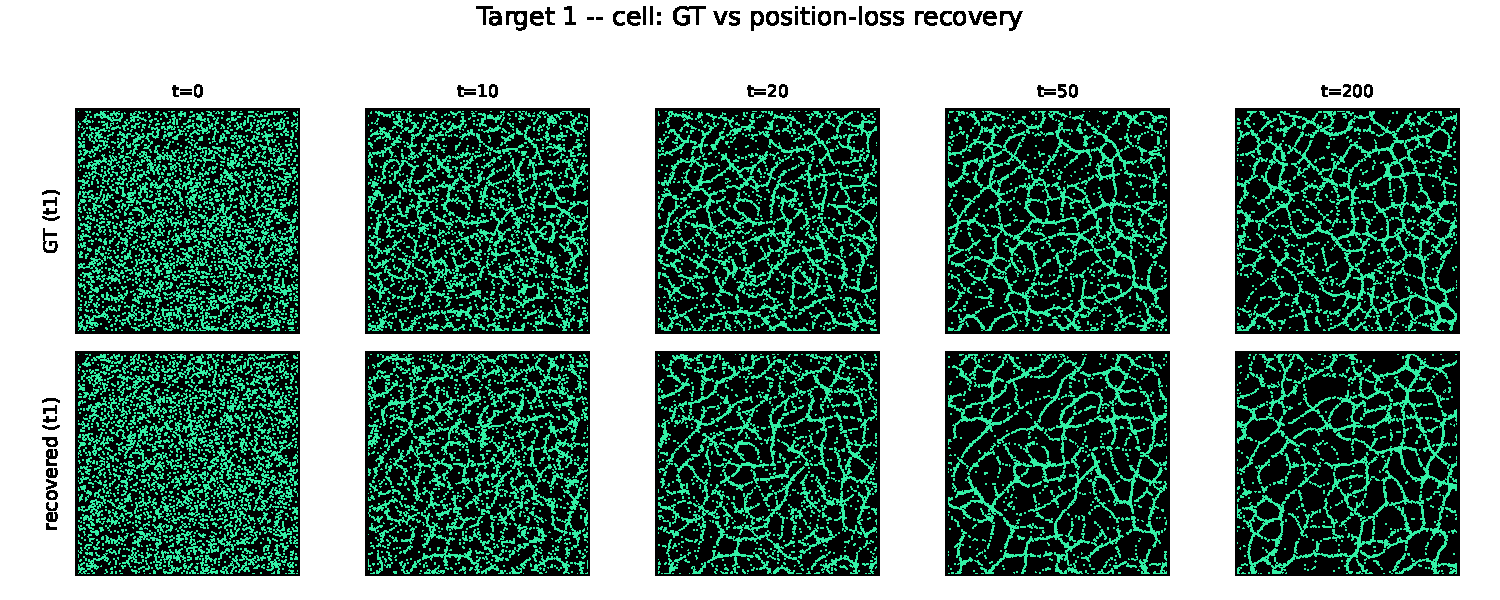
\includegraphics[width=\textwidth]{figures/gal_04.pdf}
\caption{Target 1, cell evolution: ground truth vs position-loss recovery.}
\end{figure}
\begin{figure}[p]\centering
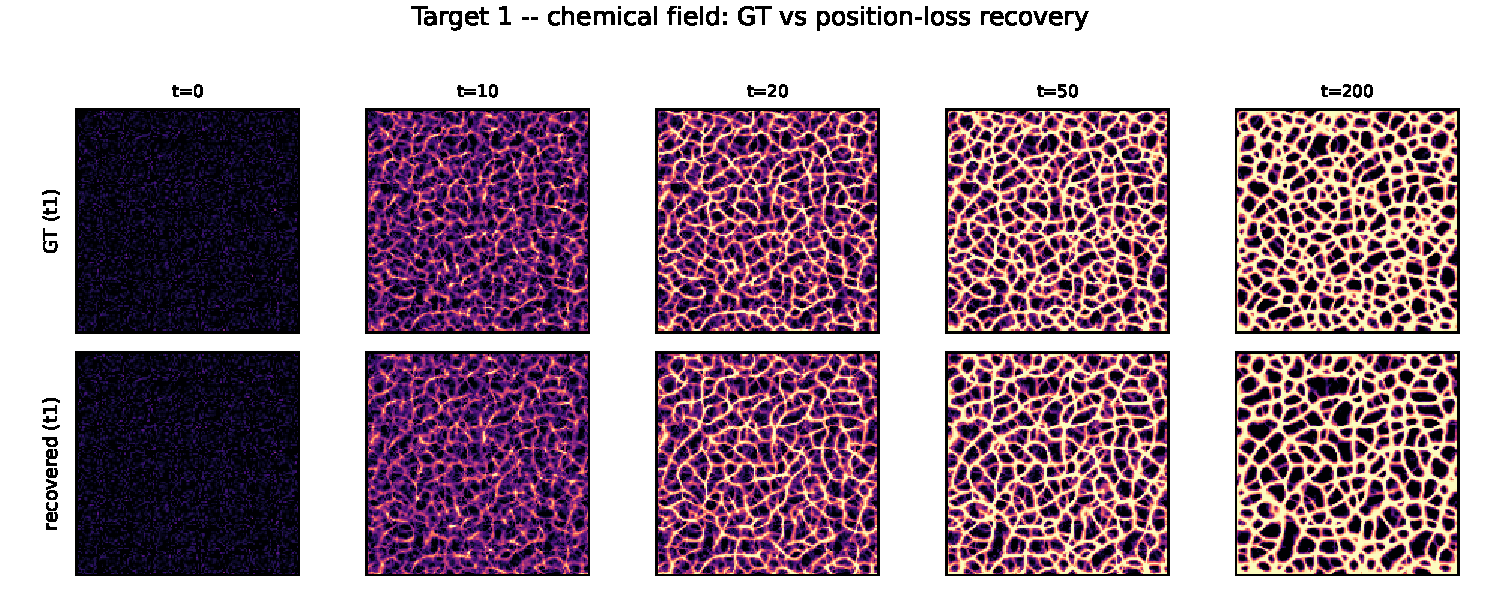
\includegraphics[width=\textwidth]{figures/gal_05.pdf}
\caption{Target 1, chemical field evolution: ground truth vs position-loss recovery.}
\end{figure}
\begin{figure}[p]\centering
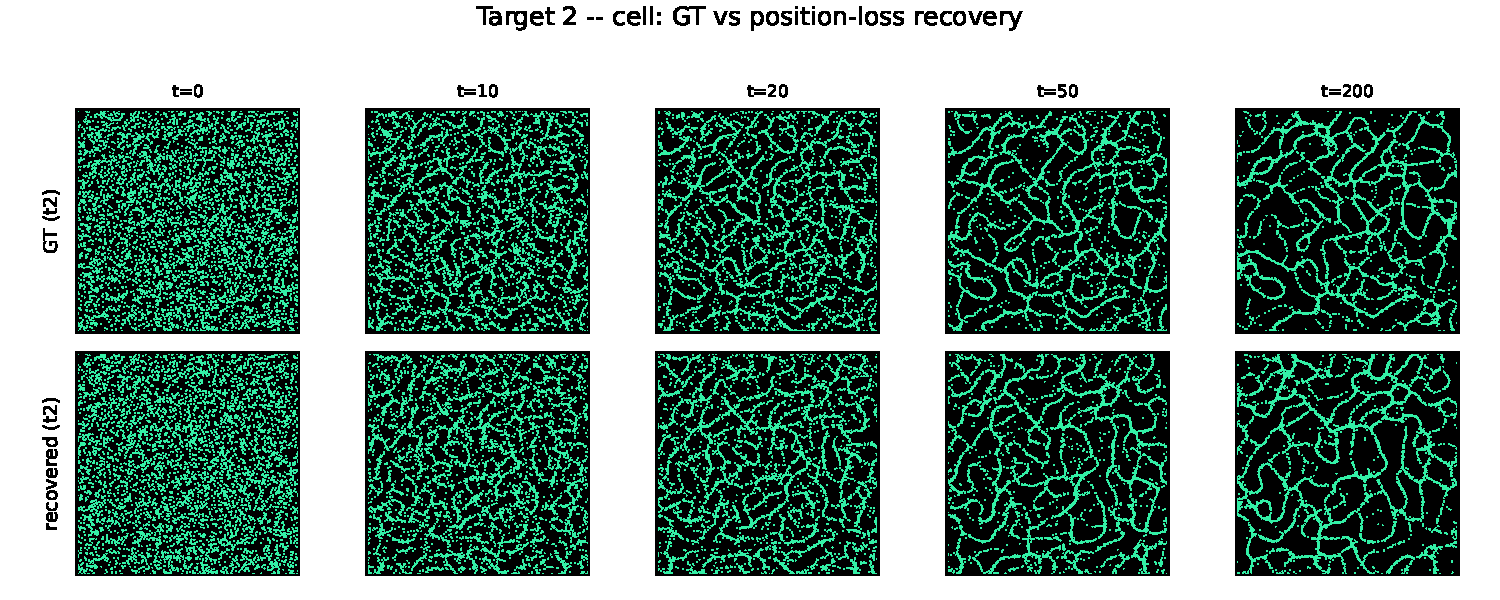
\includegraphics[width=\textwidth]{figures/gal_06.pdf}
\caption{Target 2, cell evolution: ground truth vs position-loss recovery.}
\end{figure}
\begin{figure}[p]\centering
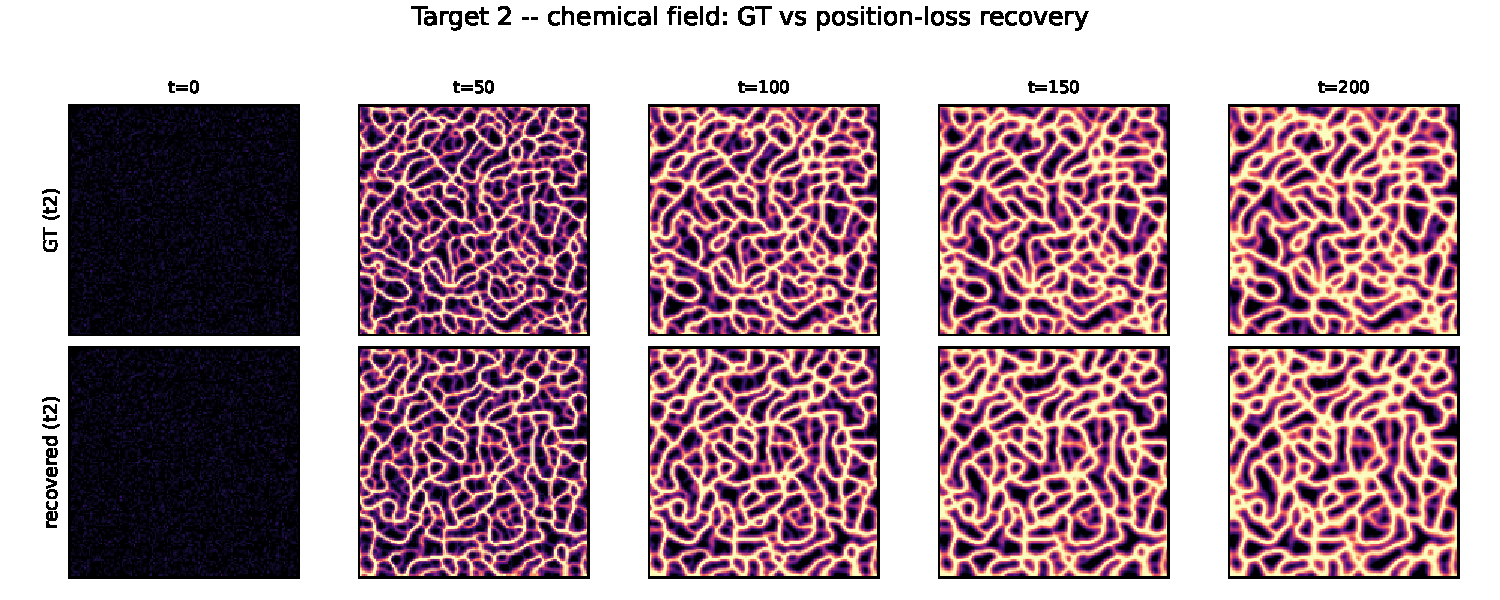
\includegraphics[width=\textwidth]{figures/gal_07.pdf}
\caption{Target 2, chemical field evolution: ground truth vs position-loss recovery.}
\end{figure}
\begin{figure}[p]\centering
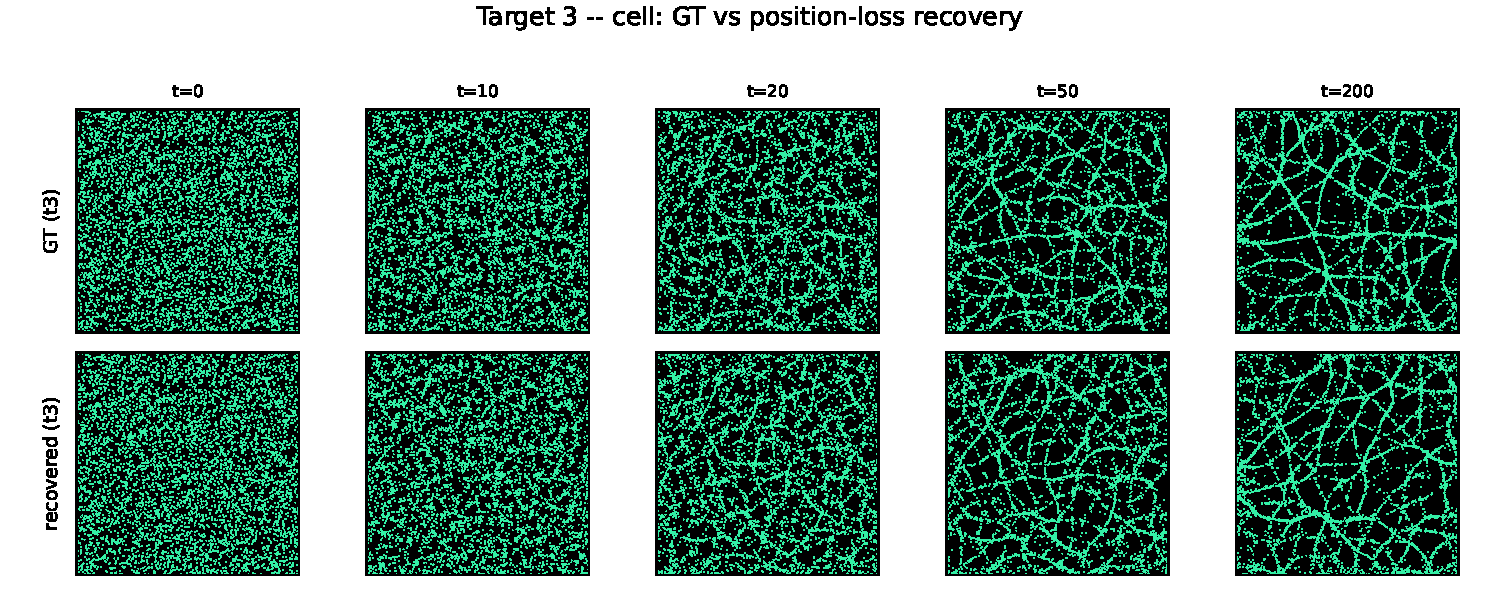
\includegraphics[width=\textwidth]{figures/gal_08.pdf}
\caption{Target 3, cell evolution: ground truth vs position-loss recovery.}
\end{figure}
\begin{figure}[p]\centering
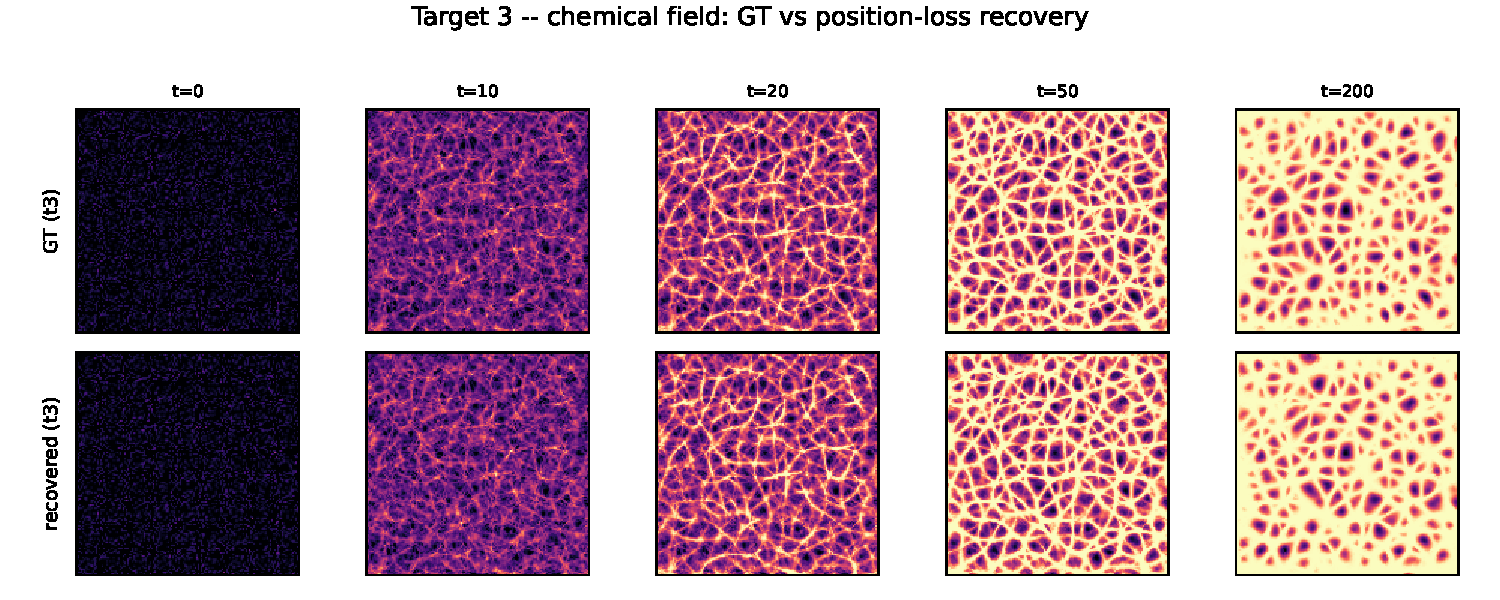
\includegraphics[width=\textwidth]{figures/gal_09.pdf}
\caption{Target 3, chemical field evolution: ground truth vs position-loss recovery.}
\end{figure}
\begin{figure}[p]\centering
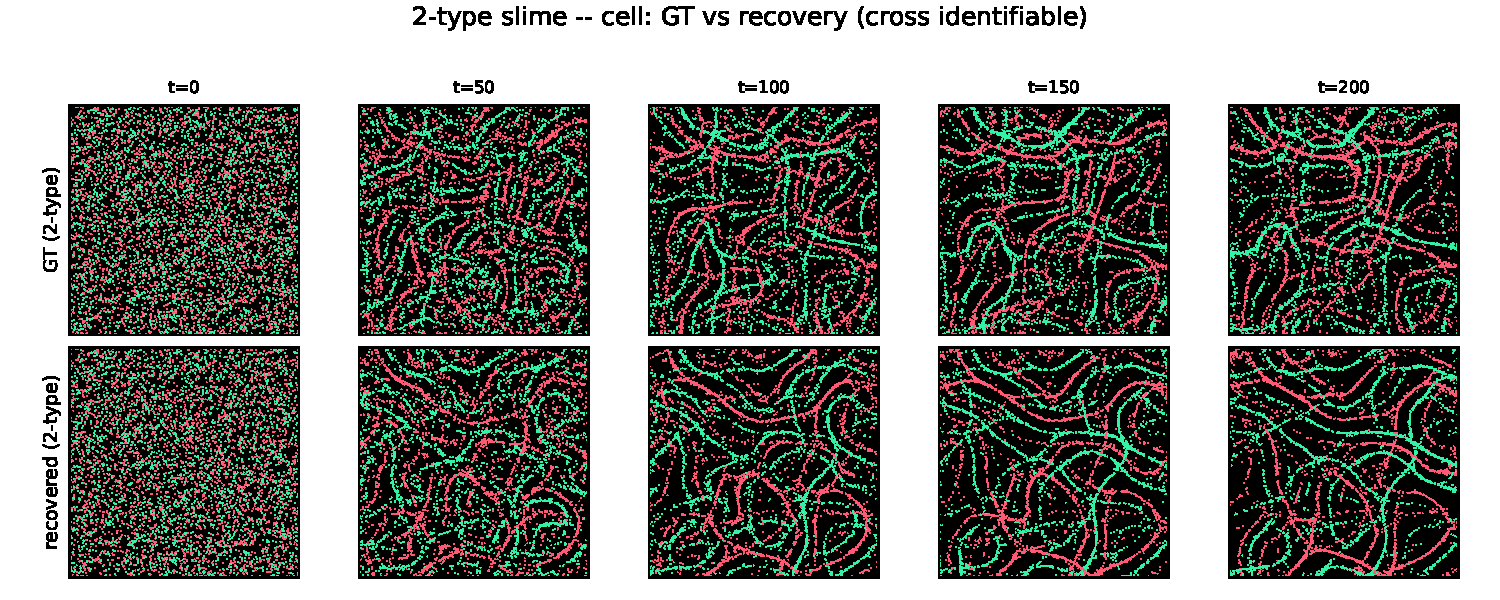
\includegraphics[width=\textwidth]{figures/gal_10.pdf}
\caption{2-type slime, cell evolution: ground truth vs recovery (cross now recovered).}
\end{figure}
\begin{figure}[p]\centering
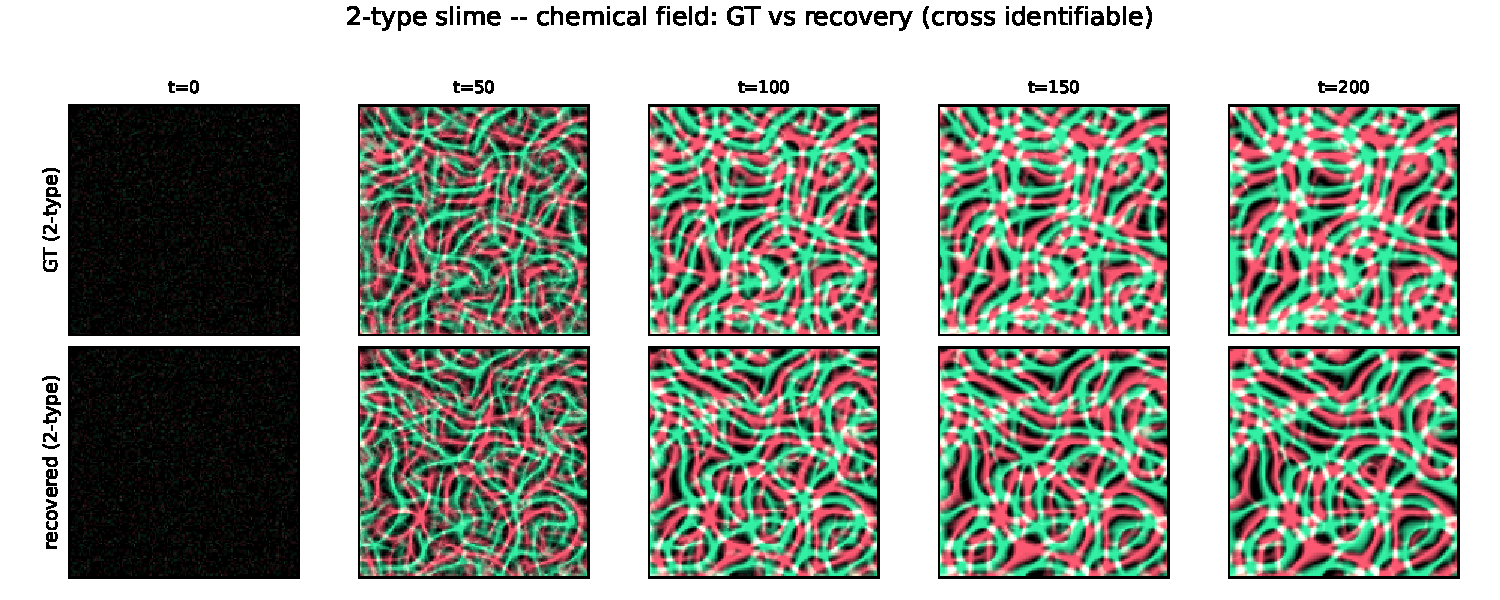
\includegraphics[width=\textwidth]{figures/gal_11.pdf}
\caption{2-type slime, chemical field evolution: ground truth vs recovery (cross now recovered).}
\end{figure}
\begin{figure}[p]\centering
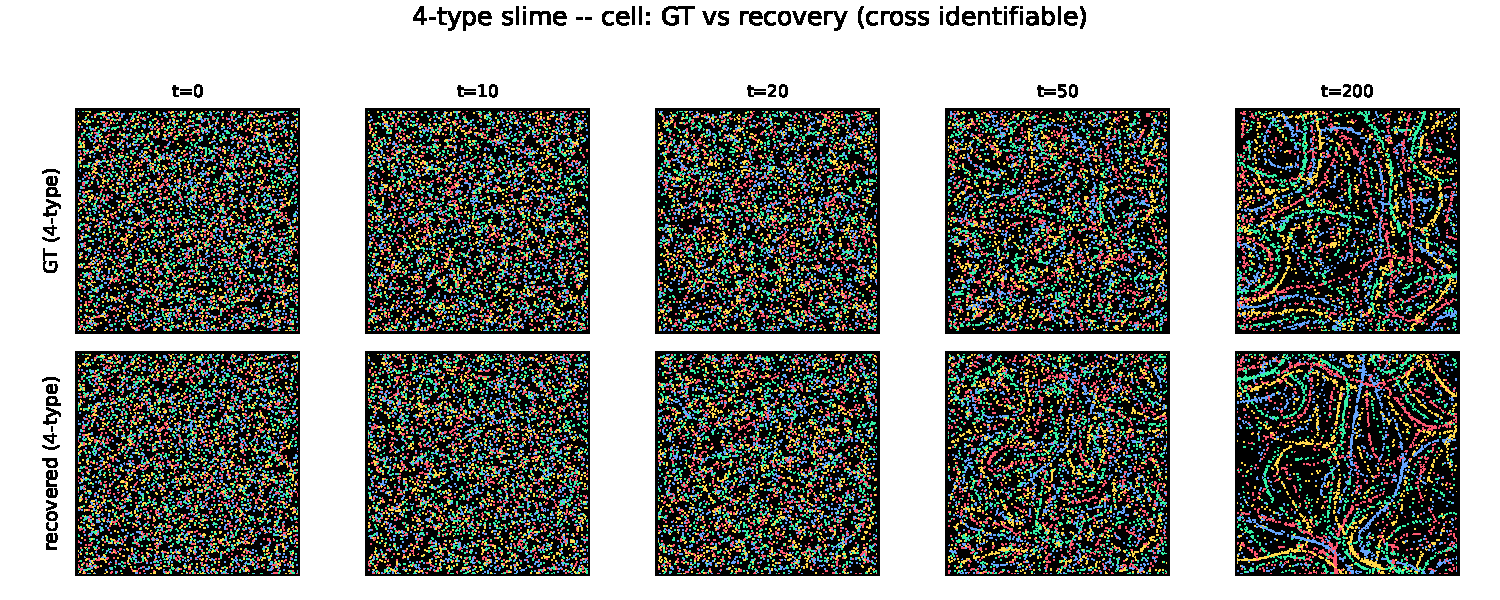
\includegraphics[width=\textwidth]{figures/gal_12.pdf}
\caption{4-type slime, cell evolution: ground truth vs recovery (cross now recovered).}
\end{figure}
\begin{figure}[p]\centering
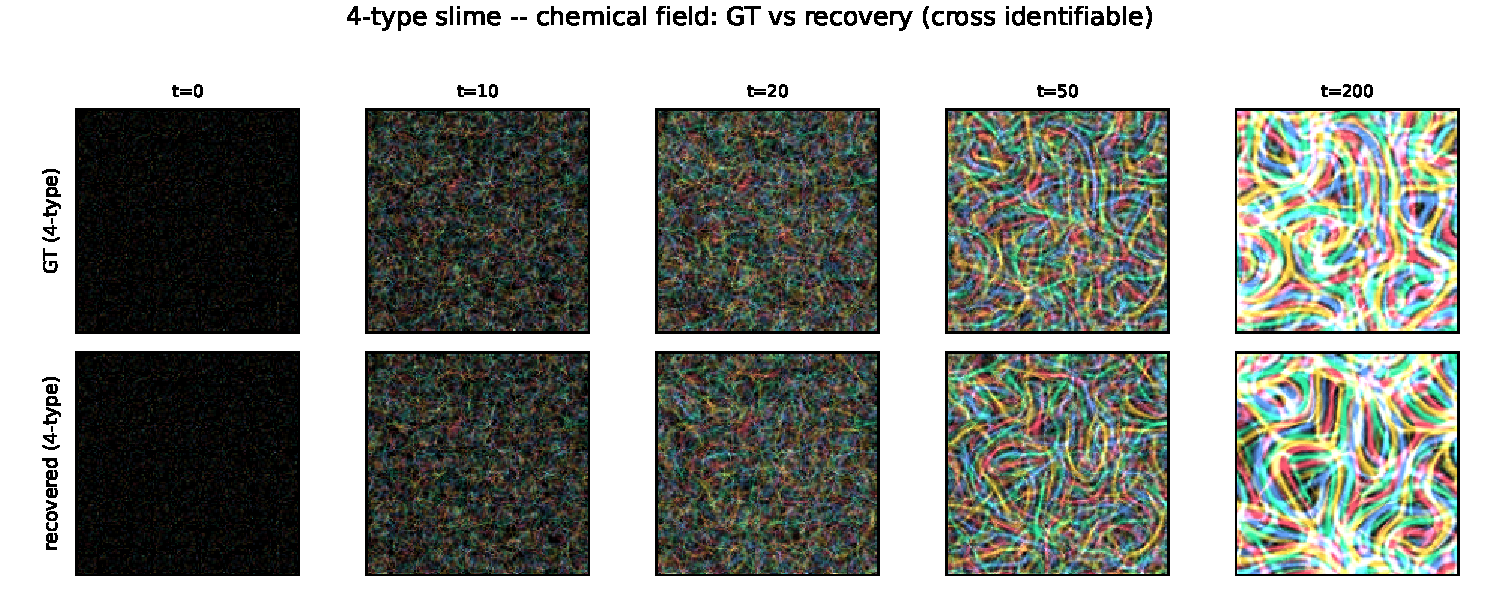
\includegraphics[width=\textwidth]{figures/gal_13.pdf}
\caption{4-type slime, chemical field evolution: ground truth vs recovery (cross now recovered).}
\end{figure}


\end{document}
